% =====================================================================
%  Dissertation Progress Report — Milestones 1 and 2
%  Compile: pdflatex twice. Overleaf-ready, no external files.
% =====================================================================
\documentclass[11pt,a4paper]{article}

\usepackage[margin=2.3cm]{geometry}
\usepackage[T1]{fontenc}
\IfFileExists{lmodern.sty}{\usepackage{lmodern}}{}
\usepackage{booktabs}
\usepackage{array}
\usepackage{xcolor}
\usepackage{listings}
\usepackage{tikz}
\usepackage{caption}
\usepackage{enumitem}
\usepackage{amsmath}
\usepackage[hidelinks]{hyperref}
\usetikzlibrary{shapes.geometric, arrows.meta, positioning, fit, backgrounds, calc}

\definecolor{navy}{RGB}{18,42,86}
\definecolor{gold}{RGB}{184,138,40}
\definecolor{softgrey}{RGB}{242,243,245}
\definecolor{midgrey}{RGB}{120,126,134}
\definecolor{good}{RGB}{22,110,72}
\definecolor{bad}{RGB}{158,42,42}
\definecolor{codebg}{RGB}{248,248,250}

\lstdefinestyle{py}{
  language=Python, basicstyle=\ttfamily\scriptsize,
  keywordstyle=\color{navy}\bfseries, stringstyle=\color{good},
  commentstyle=\color{midgrey}\itshape, backgroundcolor=\color{codebg},
  frame=leftline, framerule=1.2pt, rulecolor=\color{gold},
  xleftmargin=8pt, framexleftmargin=6pt, breaklines=true,
  showstringspaces=false, aboveskip=5pt, belowskip=5pt,
}
\lstset{style=py}

\usepackage{titlesec}
\titleformat{\section}{\normalfont\large\bfseries\color{navy}}{\thesection}{0.6em}{}
\titleformat{\subsection}{\normalfont\normalsize\bfseries\color{navy}}{\thesubsection}{0.6em}{}
\setlength{\parskip}{0.42em}
\setlength{\parindent}{0pt}

\newcommand{\up}[1]{\textcolor{good}{\textbf{#1}}}
\newcommand{\down}[1]{\textcolor{bad}{\textbf{#1}}}

\begin{document}

% ---------------------------------------------------------------- title
\begin{center}
{\LARGE\bfseries\color{navy} Spatial Mental Modeling from Limited Views}\\[4pt]
{\large Dissertation Progress Report~---~Milestones 1 and 2}\\[10pt]
{\large\bfseries Reproducing ViperGPT without Codex:}\\[2pt]
{\large\bfseries a Prompt-Specification Gap and a Depth-Reasoning Gap}\\[13pt]
\begin{tabular}{rl}
\textbf{Student} & MD Humayun \\
\textbf{Supervisor} & Dr.\ M.A. Zaveri \\
\textbf{Programme} & M.Tech CSE (Information Security and Privacy), SVNIT Surat \\
\textbf{Date} & 12 August 2026 \\
\textbf{Repository} & \texttt{mdhumayun7/Vipergpt}, tag \texttt{m2-complete} \\
\end{tabular}
\end{center}
\vspace{4pt}\hrule\vspace{9pt}

\begin{center}\begin{minipage}{0.93\textwidth}\small
\textbf{Summary.}\; ViperGPT (Sur\'is et al., ICCV 2023) answers visual queries by
prompting a code LLM to emit a Python program over vision modules. Its generator,
Codex, has been retired, so every present-day reproduction must substitute an
open-weights model. We rebuilt the pipeline end to end on an H100 cluster and report
two results. \emph{First}, the released prompt never states that a grounding program
must return an \texttt{ImagePatch}; with Qwen2.5-Coder-7B this makes \down{98.8\%} of
programs task-invalid and yields \down{0.00\%} accuracy on RefCOCO. Adding a
return-type contract and two exemplars gives \up{39.20\%} (RefCOCO) and \up{31.80\%}
(RefCOCO+). \emph{Second}, having fixed that, accuracy splits sharply by the kind of
spatial language: 2D image-plane queries reach 35.29\%, while depth and relational
queries reach \down{6.38\%}. The exposed API cannot express depth relations and the
prompt discourages geometry. That gap defines the dissertation's contribution.
\end{minipage}\end{center}
\vspace{6pt}

% =====================================================================
\section{Pipeline and what was built}

\begin{figure}[htbp]
\centering
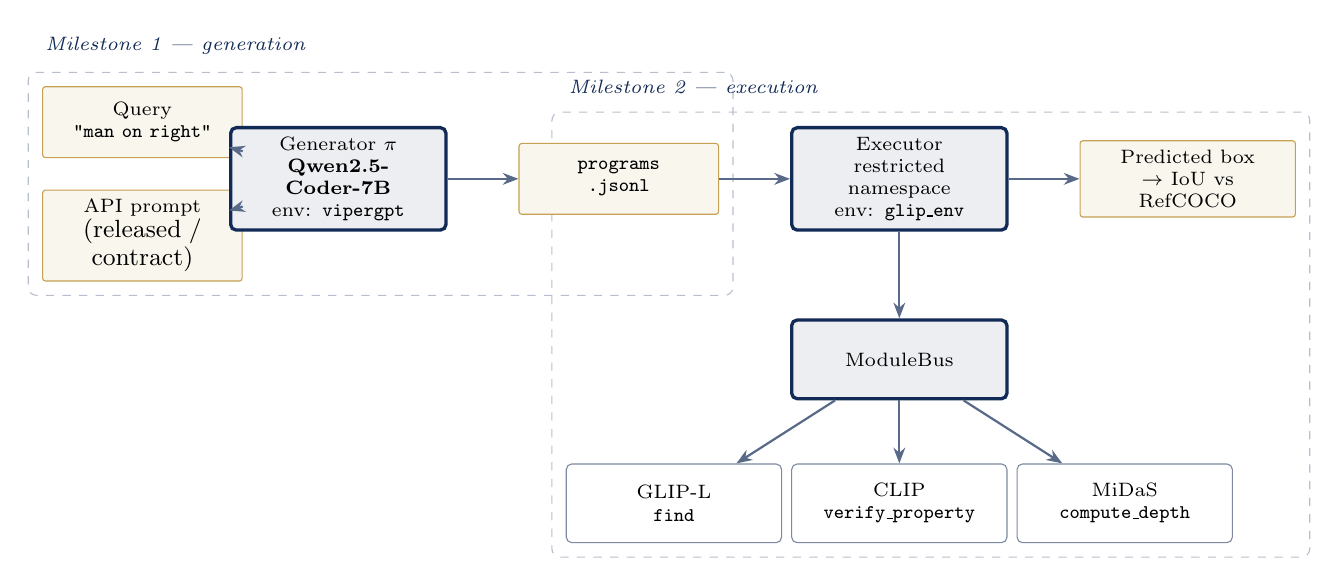
\begin{tikzpicture}[
  node distance=7mm,
  box/.style={rectangle, rounded corners=2pt, draw=navy!55, fill=white,
              text width=25mm, align=center, minimum height=10mm, font=\scriptsize},
  act/.style={box, fill=navy!8, draw=navy, very thick},
  data/.style={rectangle, rounded corners=1pt, draw=gold!80, fill=gold!8,
               text width=23mm, align=center, minimum height=9mm, font=\scriptsize},
  arr/.style={-{Stealth[length=2mm]}, draw=navy!70, thick},
  lbl/.style={font=\scriptsize\itshape, text=midgrey}
]
\node[data] (q) {Query\\ \texttt{"man on right"}};
\node[data, below=4mm of q] (pr) {API prompt\\ \small(released / contract)};
\node[act, right=11mm of $(q)!0.5!(pr)$] (gen) {Generator $\pi$\\ \textbf{Qwen2.5-Coder-7B}\\ \scriptsize env: \texttt{vipergpt}};
\node[data, right=9mm of gen] (jsonl) {\texttt{programs}\\ \texttt{.jsonl}};
\node[act, right=9mm of jsonl] (exec) {Executor\\ \scriptsize restricted namespace\\ \scriptsize env: \texttt{glip\_env}};
\node[act, below=11mm of exec] (bus) {ModuleBus};
\node[box, below left=8mm and 1mm of bus] (glip) {GLIP-L\\ \texttt{find}};
\node[box, below=8mm of bus] (clip) {CLIP\\ \texttt{verify\_property}};
\node[box, below right=8mm and 1mm of bus] (midas) {MiDaS\\ \texttt{compute\_depth}};
\node[data, right=9mm of exec, text width=25mm] (iou) {Predicted box\\ $\rightarrow$ IoU vs RefCOCO};

\draw[arr] (q) -- (gen); \draw[arr] (pr) -- (gen);
\draw[arr] (gen) -- (jsonl); \draw[arr] (jsonl) -- (exec);
\draw[arr] (exec) -- (iou);
\draw[arr] (exec) -- (bus);
\draw[arr] (bus) -- (glip); \draw[arr] (bus) -- (clip); \draw[arr] (bus) -- (midas);

\begin{scope}[on background layer]
  \node[fit=(q)(pr)(gen)(jsonl), rounded corners=3pt, draw=navy!30, dashed, inner sep=5pt] (m1b) {};
  \node[fit=(exec)(bus)(glip)(midas)(iou), rounded corners=3pt, draw=navy!30, dashed, inner sep=5pt] (m2b) {};
\end{scope}
\node[lbl, anchor=south west, text=navy] at ($(m1b.north west)+(1mm,1mm)$) {Milestone 1 — generation};
\node[lbl, anchor=south west, text=navy] at ($(m2b.north west)+(1mm,1mm)$) {Milestone 2 — execution};
\end{tikzpicture}
\caption{The reproduced pipeline. Generation and execution are split at a JSONL
boundary because the GLIP fork requires torch 2.1 while the generator runs on
torch 2.13 — the two cannot share an interpreter. The split also guarantees that
prompt conditions are compared on \emph{identical} programs.}
\label{fig:pipeline}
\end{figure}

\textbf{Infrastructure.} SVNIT HPC, 1$\times$H100 NVL per job via SLURM
\texttt{--gres=shard:N}. Building GLIP was the principal engineering risk: the
official environment pins CUDA 11.6, which has no \texttt{sm\_90} support, so the
published setup \emph{cannot run on this hardware at all}. It now builds against
torch 2.1.2/cu121 with \texttt{sm\_80;sm\_90} targets after replacing removed
\texttt{THC/*} headers in seven CUDA files and NumPy 2.0 aliases in five Python
files (D5, D6). Correctness was verified independently: the CUDA NMS kernel on a
hand-checked case, then GLIP against RefCOCO ground truth (mean IoU 0.776 at
threshold 0.2).

% =====================================================================
\section{Result 1 — the released prompt omits the grounding contract}

The released \texttt{api.prompt} is task-agnostic. Its in-context examples return
strings (\texttt{simple\_query}, \texttt{best\_text\_match}, \texttt{llm\_query}),
and nothing states that a grounding program must return an \texttt{ImagePatch}. It
further instructs: \emph{``Use base Python (comparison, sorting) for basic logical
operations, left/right/up/down, math, etc.''}

\begin{minipage}[t]{0.48\textwidth}
\textbf{Released prompt} \quad\down{invalid}
\begin{lstlisting}
# Query: "man on right"
def execute_command(image) -> str:
    image_patch = ImagePatch(image)
    man_patches = image_patch.find("man")
    if man_patches:
        man_patch = max(man_patches,
                        key=lambda m: m.right)
        return man_patch.simple_query(
            "Who is on the right?")
    return "No man found."
\end{lstlisting}
Returns a sentence. IoU undefined.
\end{minipage}\hfill
\begin{minipage}[t]{0.48\textwidth}
\textbf{+ grounding contract} \quad\up{valid}
\begin{lstlisting}
# Query: "man on right"
def execute_command(image) -> ImagePatch:
    image_patch = ImagePatch(image)
    man_patches = image_patch.find("man")
    man_patches.sort(
        key=lambda p: p.horizontal_center)
    return man_patches[-1]
\end{lstlisting}
Returns a patch. Relation resolved.
\end{minipage}

\vspace{5pt}
The intervention is three sentences stating the return type and forbidding dropped
spatial relations, plus two worked grounding exemplars. Nothing else changed.

\begin{table}[htbp]\centering\small
\caption{Effect of the grounding contract. Identical model, decoding and data;
only the prompt differs. Static columns $n=500$ per cell; execution
$n=500$ per cell.}
\label{tab:main}
\begin{tabular}{@{}lrrc@{}}
\toprule
\textbf{Metric} & \textbf{Released} & \textbf{+ Contract} & \textbf{} \\
\midrule
\multicolumn{4}{@{}l}{\itshape Static analysis of generated programs (Milestone 1)} \\
\midrule
Task-invalid return rate, RefCOCO   & 98.8\% & \up{0.2\%}  & improved \\
Task-invalid return rate, RefCOCO+  & 98.2\% & \up{0.0\%}  & improved \\
Spatial constraint dropped, RefCOCO & 17.3\% & \up{1.7\%}  & improved \\
Parse rate, RefCOCO                 & 99.8\% & \down{96.6\%} & degraded \\
Mean API calls per program          & 2.45   & 1.66        & simpler \\
\midrule
\multicolumn{4}{@{}l}{\itshape End-to-end execution, accuracy IoU $\geq0.5$ (Milestone 2)} \\
\midrule
RefCOCO / testA                     & \down{0.00\%} & \up{39.20\%} & --- \\
RefCOCO+ / testA                    & \down{0.00\%} & \up{31.80\%} & --- \\
Programs returning a patch, RefCOCO & 0 / 500 & 443 / 500 & --- \\
Programs returning a string         & 336 / 500 & 1 / 500 & --- \\
\bottomrule
\end{tabular}
\end{table}

\textbf{The zero is not a crash.} Of 500 baseline programs on RefCOCO, 336 executed
to completion and returned a \emph{string}; none returned a patch. Grounding is
scored by IoU against a box, so a sentence cannot score however correct its English.
Missing modules were ruled out as a cause: \texttt{simple\_query} and
\texttt{llm\_query} are given neutral empty-string fallbacks (D10) so that no program
can fail for lack of a module we chose not to load. That concession strictly favours
the baseline and does not change its score.

\textbf{A second, unanticipated effect.} Under the released prompt many generations
never defined \texttt{execute\_command} at all --- the model emitted prose or
malformed markdown: 136/500 (27.2\%) on RefCOCO and 214/500 (42.8\%) on RefCOCO+,
against zero under the contract. The contract disciplines output \emph{format} as
well as return type; these are separable failures and are reported separately.

\textbf{Robustness.} Greedy decoding is deterministic, so variance was estimated by
sampling ($T{=}0.7$, seeds 1--3, RefCOCO, $n{=}500$): $36.07 \pm 1.75$ against
$39.20$ greedy. Greedy beats all three sampled seeds, as expected when one program
shape is correct.

% =====================================================================
\section{Result 2 — the spatial gap, and what it is made of}

With the contract in place, accuracy splits by subset (relational-term lexicon):

\begin{table}[htbp]\centering\small
\caption{Spatial breakdown, grounding-contract condition. The baseline scores 0
everywhere and is omitted.}
\label{tab:spatial}
\begin{tabular}{@{}llrrr@{}}
\toprule
\textbf{Dataset} & \textbf{Subset} & \textbf{n} & \textbf{Accuracy} & \textbf{Mean IoU} \\
\midrule
RefCOCO  & spatial     & 289 & 35.29\% & 0.3475 \\
RefCOCO  & non-spatial & 211 & 44.55\% & 0.4378 \\
RefCOCO+ & spatial     & 47  & \down{6.38\%} & 0.1037 \\
RefCOCO+ & non-spatial & 453 & 34.44\% & 0.3474 \\
\bottomrule
\end{tabular}
\end{table}

We expected the gap to \emph{shrink} on RefCOCO+, since that dataset forbids spatial
relations. It widened threefold. A manual audit of all 47 RefCOCO+ spatial queries
explains why: the two subsets contain \textbf{different kinds of spatial language}.

\begin{center}\small
\begin{tabular}{@{}p{0.16\textwidth}p{0.36\textwidth}p{0.40\textwidth}@{}}
\toprule
 & \textbf{RefCOCO} & \textbf{RefCOCO+} \\
\midrule
Type & 2D image-plane & depth and inter-object \\
Examples & \emph{man on right}, \emph{person bottom left} & \emph{man closest to us},
\emph{farthest man}, \emph{umpire behind catcher} \\
Resolvable by & sorting patch coordinates in base Python & requires
\texttt{compute\_depth} or 3D geometry \\
Accuracy & 35.29\% & 6.38\% \\
\bottomrule
\end{tabular}
\end{center}

\vspace{4pt}
Forbidding spatial language removed viewer-frame \emph{directional} expressions and
left depth-ordering and relational ones. The released prompt's instruction to use
base Python for ``left/right/up/down'' works for the first and cannot work for the
second. Consistently, Milestone 1 found \texttt{compute\_depth} invoked 29 times
against 547 for \texttt{find} and 5 for \texttt{distance}: the geometric API is
effectively unused, by design of the prompt.

Two further observations support this reading. All three successes in the RefCOCO+
spatial subset are depth queries with very high IoU (0.97, 0.96, 0.92) --- when depth
ordering \emph{is} attempted correctly, localisation is excellent; it is usually not
attempted. And across seeds, spatial variance is roughly four times non-spatial
variance ($\pm3.35$ vs $\pm0.72$): programs handling spatial relations are not merely
less accurate but less \emph{stable}, sometimes resolving a relation by sorting and
sometimes dropping it entirely.

\textbf{Caveat.} $n{=}47$, so 6.38\% is 3 of 47 and the interval is wide. The lexicon
also produces roughly five false positives in that subset, which would push true
depth-query accuracy lower still. The direction is informative; the value is not.

% =====================================================================
\section{Reproducibility record}

\begin{center}\small
\begin{tabular}{@{}p{0.05\textwidth}p{0.30\textwidth}p{0.57\textwidth}@{}}
\toprule
\textbf{ID} & \textbf{Deviation} & \textbf{Reason / effect} \\
\midrule
D1 & Codex $\rightarrow$ Qwen2.5-Coder-7B & Codex retired; no faithful option. The
substitution is what exposes Result 1, and is the dominant term in the gap to 72.0. \\
D2 & Scope: grounding only & GQA/OK-VQA/NExT-QA need $\sim$250\,GB against 231\,GB
quota; OK-VQA also needs GPT-3, likewise retired. \\
D3 & RefCOCO annotations from Internet Archive & The canonical UNC host no longer
resolves. Archived zips are byte-identical. No effect. \\
D5, D6 & GLIP built for sm\_90 & CUDA 11.6 has no sm\_90. Headers and NumPy aliases
updated; kernels unchanged. Verified numerically. \\
D8 & GLIP threshold $0.2$ (paper unspecified) & Swept on 20 samples: 0.5 loses 8/20
detections, 0.2 gives mean IoU 0.776. Material and under-validated. \\
D9 & X-VLM $\rightarrow$ CLIP & X-VLM weights are Google-Drive-only. CLIP scores
globally, so attribute checks are weaker --- costliest on RefCOCO+. \\
D10 & \texttt{simple\_query}/\texttt{llm\_query} return \texttt{""} & Loading
BLIP-2-XXL and an 8B text LLM is out of scope. Favours the baseline; no effect on the
contract condition. \\
\bottomrule
\end{tabular}
\end{center}

\vspace{4pt}
\textbf{Two recorded failures.} A first hypothesis --- that spatial queries would
collapse into a single opaque \texttt{simple\_query} call, as the paper's GQA prompt
instructs --- was tested and rejected (collapse rate $\approx0\%$); that instruction
applies to GQA, and grounding cannot use \texttt{simple\_query} because it must
return a patch. Separately, an early 500-sample execution ran on a login node with no
GPU, producing a complete and entirely fake results table; those runs were deleted
and job scripts now assert \texttt{torch.cuda.is\_available()}. Silent CPU fallback
is the most dangerous failure mode encountered, because it yields plausible output
rather than an error.

\textbf{Artefacts.} Every run writes a timestamped directory with resolved config,
per-query programs, per-sample records and a summary; SLURM job IDs are recorded;
\texttt{docs/research\_log.md} (540+ lines) documents the full arc including failures.

% =====================================================================
\section{Where the gap to 72.0 comes from}

Reproduced 39.20 against a reported 72.0. Raw GLIP top-box accuracy on this data is
78.9\%, so perception caps the system near 79\% before any program runs; program-level
selection loses roughly 40 points from there. Ordered by likely size, the
contributors are D1 (generator substitution, dominant), the perception ceiling,
D9 (X-VLM$\rightarrow$CLIP, costliest on RefCOCO+, consistent with 31.80 vs 39.20),
and D8 (threshold tuned on 20 samples). No claim of a faithful reproduction is made:
what is reproduced is the method; what is measured is what happens to it when its
generator is replaced.

% =====================================================================
\section{Proposed contribution}

The measured problem is specific: \emph{the API cannot express depth relations, and
the prompt discourages geometry}. \texttt{compute\_depth()} returns one scalar --- the
median relative depth of a patch --- from which ``A is behind B'' is expressible but
``the third-closest person'', ``between A and B in depth'', and metric size are not.

\textbf{Proposal.} Replace the scalar with a back-projected representation and expose
operations over it: \texttt{position\_3d}, \texttt{depth\_order},
\texttt{is\_behind}, \texttt{distance\_3d}, \texttt{is\_between\_3d},
\texttt{physical\_size}; swap MiDaS for a metric depth model; and remove the
anti-geometry instruction from the prompt. \texttt{depth\_order} is the
highest-value single primitive --- \emph{closest}, \emph{nearest}, \emph{farthest}
account for most of the audited subset.

\textbf{Evaluation} reuses the existing pipeline unchanged. Three conditions:
released prompt (0.00\%), grounding contract (39.20\% / 6.38\% on depth queries), and
the depth-grounded API. The primary claim is improvement on the depth subset; the
necessary control is that the 2D subset and non-spatial sets do not degrade. The
paper's own interventional protocol (Sec.\ 5.2) applies: neutralising
\texttt{depth\_order} must cause a measurable drop, or the primitive is decorative.
A prompt-only ablation separates \emph{encouraging} geometry from \emph{providing} it.

\textbf{Honest risk.} The generator may ignore the new API as it ignores
\texttt{compute\_depth} today. Call frequency will therefore be measured directly, as
in Milestone 1. If the API is not invoked, the finding concerns prompt adherence
rather than geometry --- still reportable, but weaker.

Metric depth is claimed only as \emph{ordering}: COCO has no camera intrinsics, so
absolute metres would rest on an assumed field of view. \texttt{depth\_order} and
\texttt{is\_behind} require only monotonicity, which relative depth already provides.

% =====================================================================
\section{Limitations and next steps}

\begin{enumerate}[leftmargin=1.3em, itemsep=2pt]
\item One generator (Qwen2.5-Coder-7B). Whether the prompt effect is scale-dependent
is untested; a 1.5B/32B sweep needs no new infrastructure.
\item GLIP threshold tuned on 20 samples (D8); to be re-swept before final numbers.
\item X-VLM substituted by CLIP (D9); the substitution most likely to be costing
accuracy, especially on RefCOCO+.
\item Seed variance measured on RefCOCO only, and by sampling rather than by
retraining --- the standard caveat for a decoding-only estimate.
\item Spatial subsets are identified by lexicon, not human annotation.
\end{enumerate}

\vspace{8pt}\hrule\vspace{3pt}
{\footnotesize\color{midgrey}
All figures traceable to a run directory, an archived summary in
\texttt{results/m2\_summaries/}, and a SLURM job ID. Milestone 1: jobs 29187, 29193.
Milestone 2: jobs 29290, 29292, 29301, 29306. Repository tags
\texttt{m1-complete}, \texttt{m2-glip-verified}, \texttt{m2-execution},
\texttt{m2-complete}.}

\end{document}
